\chapter{Desarrollo}

En este capítulo se explicará las fases del desarrollo basado en prototipos en las que incrementalmente se implementan la funcionalidades del sistema.

Para esto, se considera el uso de contenedores virtualizados con \textbf{Docker} para construír los servicios de cada componente del chatbot. En este proyecto estos servicios quedarán definidos en un archivo \href{https://github.com/AranGarcia/milo-bot/blob/master/docker-compose.yml}{docker-compose.yml} lo cuál permitirá fácilmente la construcción y despliegue de estos servicios. En este archivo se definen los siguientes servicios:

\begin{itemize}
    \item Fuente de almacenamiento de datos
    \item Servidor HTTP para atender peticiones del cliente web
    \item Ejecución e interpretación de los mensajes de texto del usuario.
\end{itemize}

Utilizando el archivo de configuración de servicios Docker y el orquestador \textbf{Docker Compose}, todos los servicios se pueden inicializar con la instrucción:

\begin{lstlisting}[language=bash]
  $ docker-compose up
\end{lstlisting}

\section{Primera iteración}

\subsection{Extracción de Texto de los Documentos del Marco Normativo}

Como se mencionó en la sección \ref{subsec:marco-normativo-ipn}, el IPN ofrece accesibilidad al conjunto de documentos que conforman el marco normativo. Existe un problema en utilizar estos documentos como fuente de información para el sistema propuesto en este trabajo terminal: \textbf{la divulgación de estos documentos se hacen en formato PDF}. Los formatos PDF agregan un formato de organización gráfica y visual, pero no son óptimos para procesos de extracción.


\begin{figure}[ht]
    \centering
    \fbox{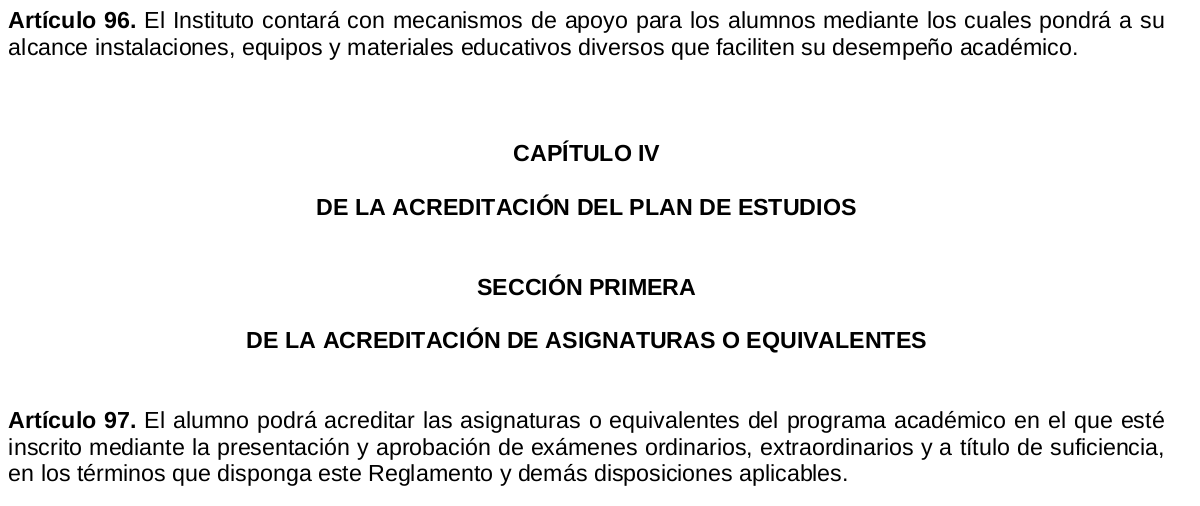
\includegraphics[scale=0.38]{6/ejemplo_reglamento_1}}
    \caption{Segmento del Reglamento Interno del Instituto Politécnico Nacional}
    \label{fig:ejemplo_1_reglamento_interno}
\end{figure}

\begin{figure}[ht]
    \centering
    \fbox{
\includegraphics[scale=0.39]{6/ejemplo_reglamento_2}}
    \caption{Segmento del Reglamento Orgánico del Instituto Politécnico Nacional}
    \label{fig:ejemplo_2_reglamento_organico}
\end{figure}

\begin{figure}[ht]
    \centering
    \fbox{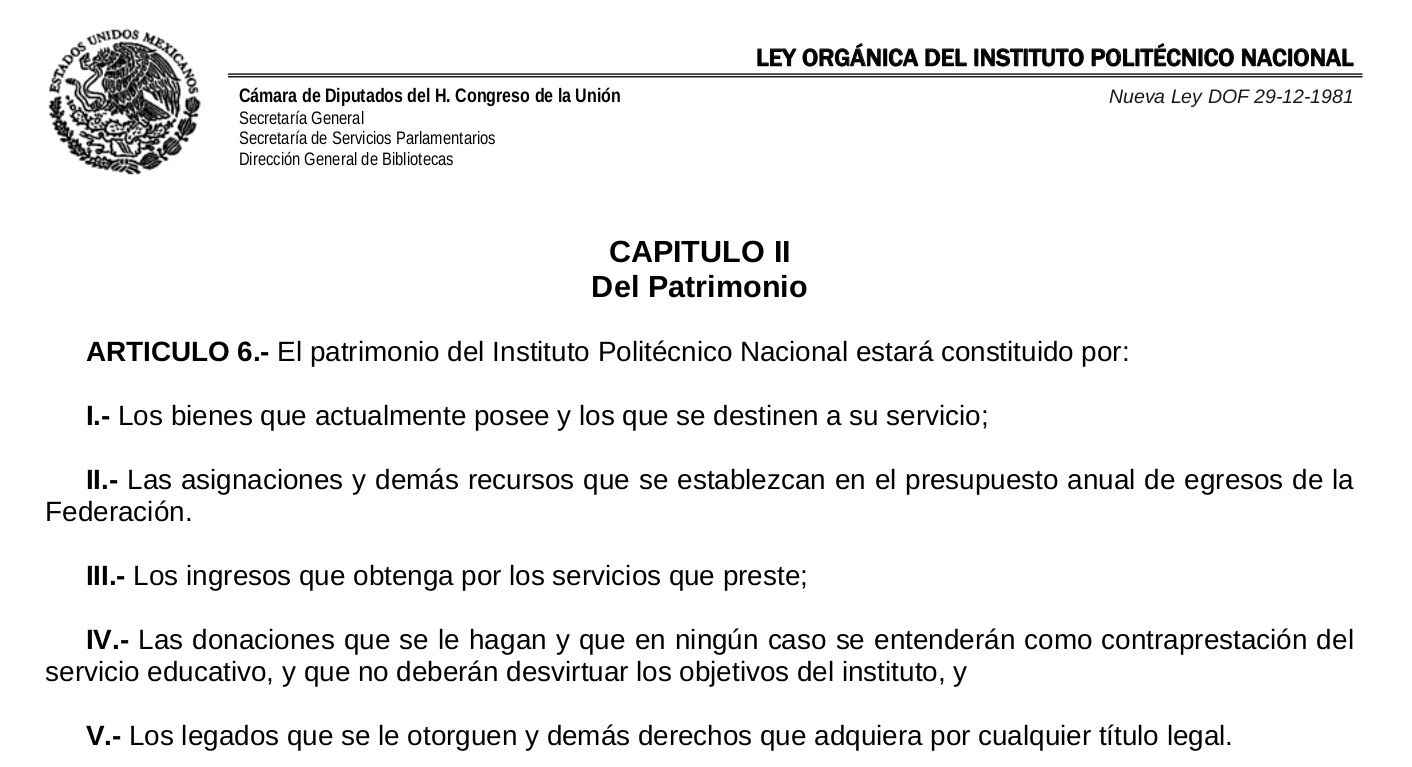
\includegraphics[scale=0.32]{6/ejemplo_reglamento_3}}
    \caption{Segmento de la Ley Orgánica del Instituto Politécnico Nacional}
    \label{fig:ejemplo_3_ley_organica}
\end{figure}

El problema general es este: la figura \ref{fig:ejemplo_1_reglamento_interno} muestra una manera muy sencilla de organización textual de la información, pero difiere mucho en cuanto a la organización de contenido de la figura \ref{fig:ejemplo_2_reglamento_organico}. Mas aún, la figura \ref{fig:ejemplo_3_ley_organica} añade a la estructura de la página una cabecera con nombres de una institución y sus direcciones internas, las cuáles son irrelevantes en cuanto al contenido normativo de nuestro interés.
 
Por lo tanto, podemos concluir que un estándar de división estructural normativa no es suficiente en sí, sino también \textbf{se debe estandarizar la forma en cómo se representan esos datos cuando se almacenan}. Esto es un problema de \textbf{serialización} de datos en la que no existe un formato unificado semántico. Se debe extraer esta información para posteriormente unificar su formato. Esto es el siguiente paso de la preparación del texto.

A pesar de que son relativamente pocos documentos, la cantidad de texto contenido dentro de ellos es grande como para extraer de manera manual. Sin embargo, para este trabajo terminal se ha decidido \textbf{extraer el texto a mano}. Este método es muy inconveniente por diversas razones. La principal razón que se considera en el desarrollo de este trabajo terminal es por el esfuerzo manual requerido, el cuál hace que el proceso sea propenso a errores. Como consecuencia esto también la cantidad de tiempo invertida en desarrollar este trabajo terminal.

Sin embargo, si se depende de una herramienta que extraiga texto automática mente, resulta en incongruencias como el siguiente segmento de texto extraído de la figura \ref{fig:ejemplo_2_reglamento_organico}:

\begin{quote}
    \textbf{Artículo 10.} En caso de que algún miembro del person-gación, al desarrollo y fomento tecnoloógico y empre-nal del Instituto reciba el nombramiento de directivo en sarial, o unidad educativa vinculada a ciencia, tecnología...
\end{quote}

Esto es debido a que la organización de texto no es la misma que la organización visual de un documento PDF. En este caso, la herramienta de extracción de PDF lo hizo por cada renglón de la página, sin importar que el documento estuviera dividido en dos columnas.

\newpage
\subsubsection{Formato de Documento Normativo de Entrada}

Entonces necesitamos que el documento venga en formato TXT, y que cada \textbf{título}, \textbf{sección}, \textbf{capítulo} y \textbf{artículo} venga separado por dos saltos de línea (\textbackslash n\textbackslash n). Tambien el texto y el nivel estructural debe ser separado con un guin (-) o un punto (.).

\begin{quote}
    \textbf{Capítulo Primero} - Disposiciones Generales
    
    \textbf{Artículo 1}. Las disposiciones del presente Reglamento son de observancia general y obligatoria en el Instituto Politécnico Nacional.
    
    \textbf{Artículo 2}. Este ordenamiento tiene por objeto establecer las condiciones que regulan el ingreso, la trayectoria escolar, la permanencia y el egreso de alumnos que cursen algún programa académico de los niveles medio superior, superior y posgrado, así como de los usuarios de todos aquellos programas que se ofrezcan para complementar su formación y con fines de capacitación, actualización técnica y profesional, formación empresarial, educación continua, y enseñanza de lenguas extranjeras en las unidades académicas, unidades de apoyo a la innovación educativa, unidades de apoyo a la investigación y al fomento y desarrollo empresarial y demás áreas referidas en el artículo 2 del Reglamento Orgánico, en las modalidades educativas que ofrece el Instituto Politécnico Nacional.
    
    \textbf{Artículo 3}. Para efectos del presente Reglamento se entenderá por:
    Academia: Al órgano constituido por profesores que tiene la finalidad de proponer, analizar, opinar, estructurar y evaluar el proceso educativo.
    ...
\end{quote}

Por ejemplo:

\begin{itemize}
    \item El primer elemento sería el capítulo primero, se separa el texto de su nivel mediante el guión. Posteriormente se introducen dos saltos de línea para separarlo del artículo 2. 
    \item El tercer elemento es el artículo 3. Este tiene mas de un párrafo, por lo que un solo salto de línea separa sus párrafos pero no lo separa del artículo siguiente hasta que encuentre los dos saltos de línea.
\end{itemize}

Los documentos normativos extraidos manualmente a un formato TXT se pueden encontrar en el siguiente repositorio: \url{https://github.com/AranGarcia/Shepard}.

\subsubsection{Estructura Propuesta}

Una vez obtenido el formato TXT de entrada, se utilizará como entrada al sistema para su almacenamiento en la base de conocimiento.

Para estructurar los reglamentos, se toma en cuenta la jerarquía de su división estructural mientras se mantenga el contenido textual así como la enumeeración. Es por eso que se propone la siguiente estructura:

\begin{itemize}
    \item \textbf{items}: arreglo de objetos con los siguientes atributos:
    
    \begin{itemize}
        \item \textbf{contenido}: objeto anidado recursivo
        
        \begin{itemize}
            \item \textbf{items}: ...
            \item \textbf{nivel}: ...
        \end{itemize}
        
        \item \textbf{enumeracion}: número de elemento de la división estructural
        \item \textbf{texto}: contenido textual del elemento
    \end{itemize}
    
    \item \textbf{nivel}: nombre del nivel de la división estructural
\end{itemize}

Este formato es para mantener una forma jerárquica inherente en los documentos normativos discutidos anteriormente y que se les denomina divisón estructural. Entonces se desarrollará un programa que dado un documento normativo TXT lo transforme a la estructura propuesta.

\begin{figure}
    \centering
    \lstinputlisting[language=JSON]{src/3/ejemplo-estructura.json}
    \caption{Estructura propuesta inicialmente para organizar texto mediante el formato JSON.}
    \label{fig:estructura_propuesta}
\end{figure}

El programa que realiza esto se puede encontrar en el repositorio \url{https://github.com/AranGarcia/Cookie/tree/master/yamlizer}.



\subsection{Construcción del Cliente e Interfaz Web}

La interfaz web se implementó con base a la definición de su diseño en la sección \ref{subsubsec:ui-entorno-chat}. Inicialmente, solo utiliza el cliente para poder cumplir con los casos de uso definidos en la sección \ref{sec:casos-de-uso}, es decir, verificar la disponibilidad del servicio del chatbot.

La figura \ref{fig:interfaz-web-falla} muestra una captura de pantalla la interfaz implementada junto con el cliente web que se encargará de hacer peticiones para el chatbot. Inicialmente, sin el servicio del chatbot el cliente web mostrará mensajes indicando que es imposible atender peticiones en ese momento.

Sin embargo, también se desea mostrar el caso exitoso en el que la conversación sigue el guión deseado. Para ello, se implementó un servicio de prueba en donde el cliente solo se encarga de verificar el estado del servicio del chatbot mediante una petición \textit{health check} al puerto \textbf{5055} y el servidor devuelve una respuesta HTTP con estado \textbf{200 OK}. Esto hace que el cliente ejecute la trayectoria deseada de inicialización, como se puede ver en la figura \ref{fig:interfaz-web-exito}.

\begin{figure}
    \centering
    \fbox{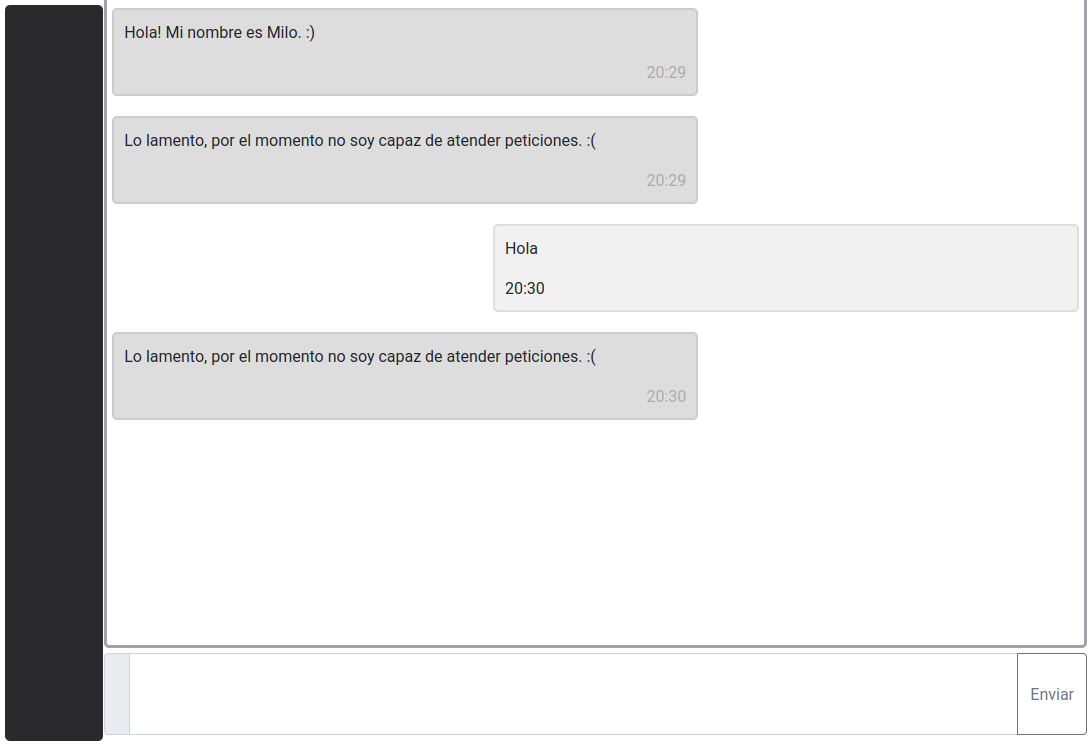
\includegraphics[scale=0.4]{images/6/interfaz-web-falla}}
    \caption{Inicialización del cliente: falla al intentar establecer conexión.}
    \label{fig:interfaz-web-falla}
\end{figure}

\begin{figure}
    \centering
    \fbox{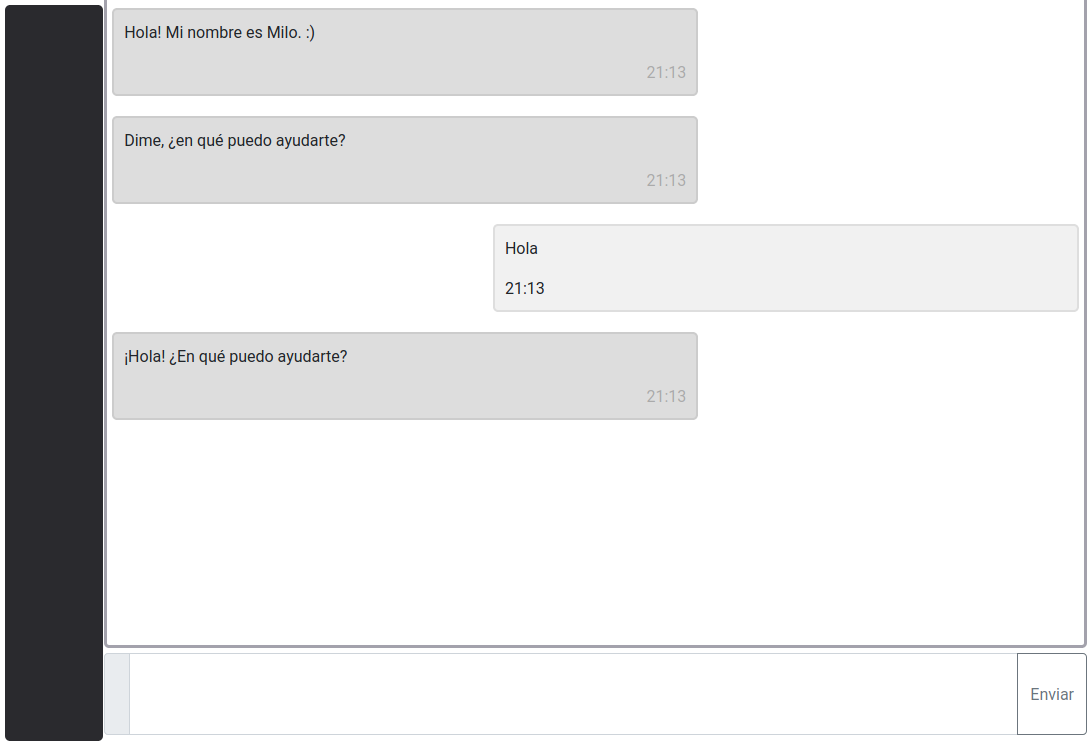
\includegraphics[scale=0.4]{images/6/interfaz-web-exito}}
    \caption{Interfaz web: conexión exitosa con el servicio del chatbot.}
    \label{fig:interfaz-web-exito}
\end{figure}

\subsection{Construcción del modelo de datos inicial}

Se eligió PostgreSQL como gestor de base de datos que aloja la base de conocimientos de los documentos normativos. En el directorio \href{https://github.com/AranGarcia/milo-bot/tree/master/db}{db/} se podrá encontrar la definición del servició y el esquema de la base de datos implementado.

Una vez definido el modelo de datos para alojar la base de conocimientos, se debe implementar el proceso de transformación y carga de datos para la base de conocimientos.

\section{Segunda iteración}  

\subsection{Preparación del Intérprete}

El framework \textbf{Rasa} proporciona herramientas para la configuración de modelos conversacionales que se entrenan a partir de datos de entrenamiento introducidos como muestra, así como también un SDK para poder implementar acciones personalizadas.

Como ya se estableció en el diseño, la generación de una respuesta requiere que se determine que la intención del usuario sea 1 de 4 posibles categorías mutuamente excluyentes:

\begin{itemize}
    \item \verb|saludar|
    \item \verb|despedir|
    \item \verb|extraer_articulo|
    \item \verb|buscar_conceptos|
\end{itemize}

En la figura \ref{fig:actividad-responder} se indica que cuando se cumpla la condición que la intención sea \verb|extraer_articulo|, se deba extraer el reglamento dado su ubicación en un documento. Esto se hace también fijando como objetos para el aprendizaje las siguientes entidades:

\begin{itemize}
    \item \verb|documento|: uno de los documentos normativos del cual el chatbot tendrá conocimiento.
    \item \verb|nivel_estructural|: identifica si es cualquiera de los niveles de la división estructural normativa que existen, ya sea título, capítulo, sección o artículo.
    \item \verb|enumeracion|: el numero correspondiente del nivel que se desea encontrar.
\end{itemize}

\subsection{Proceso de aprendizaje}

Para poder entrenar el modelo de entendimiento de lenguaje natural con \textbf{Rasa} necesitamos tres cosas:

\subsubsection{Datos de entrenamiento}

El aprendizaje debe tener un buen conjunto de datos lo suficientemente disperso para que el clasificador identifique las estructuras esenciales de cada mensaje para determinar su intención y las entidades. Por ejemplo, para la intención de extraer un artículo, el conjunto de entrenamiento contiene instancias con una estructura similar a estas oraciones:

\begin{itemize}
    \item \textit{"Dame el contenido del articulo nivel estructural  2 de la ley orgánica."}
    \item \textit{"Muéstrame el contenido del articulo 2 del reglamento interno."}
    \item \textit{"¿Qué dice el articulo 2 del reglamento general de estudios?"}
\end{itemize}

Todo esto se podrá encontrar en el archivo \href{https://github.com/AranGarcia/milo-bot/blob/master/rasa/data/nlu.yml}{rasa/data/nlu.yml} Así mismo, también el conjunto de datos debe tener etiquetado de las características esenciales que buscamos reconocer, lo cuál se explican mas adelante en la definición de los tipos de datos.

\subsubsection{Configuración del modelo de aprendizaje}

El framework proporciona una manera de configurar los procesos de aprendizaje a través del archivo \href{https://github.com/AranGarcia/milo-bot/blob/master/rasa/config.yml}{rasa/config.yml}. Dentro de esta configuración, se establece múltiples procesos comúnmente usados como generadores de tokens y analizadores de características sintácticas. Cabe mencionar que el componente clave que ayuda a la clasificación de intención y extracción de entidades es el transformador \href{https://rasa.com/docs/rasa/components#dietclassifier}{DIET} (Dual Intent and Entity Transformer).

\textbf{Nota}: Ya que el propósito principal es la búsqueda de conceptos similares en el corpus de texto, se hará que la intención \verb|buscar_conceptos| sea la acción por defecto con un los siguientes parámetros:
\begin{itemize}
    \item \verb|threshold|: El umbral general de certidumbre. Si ninguna intención obtiene una certeza mayor a este umbral, automáticamente se elige la acción por defecto.
    \item \verb|ambiguity_threshold|: Con este parámetros, especificamos si la diferencia entre las dos intenciones clasificadas como las mas altas tienen una diferencia menor o igual a este valor, entonces elegirá la intención por defecto.
\end{itemize}

\subsubsection{Definición de los tipos de datos}

En esta parte se definen las categorías posibles para una intención y las entidades que conforman a cada tipo de mensaje, las cuales ya se han mencionado. Esto se ha configurado en el archivo \href{https://github.com/AranGarcia/milo-bot/blob/master/rasa/domain.yml}{rasa/domain.yml}.

Las entidades que reconocerá el clasificador DIET de Rasa son las siguientes:t
\begin{itemize}
    \item \textbf{documento}: Tiene un tipo de dato texto categórico; es decir, puede ser uno de los siguiente: \textit{reglamento general de estudios}, \textit{ley organica}, \textit{reglamento de titulacion} o \textit{reglamento interno}.
    \item \textbf{nivel\_estructural}: Texto categórico que puede ser uno de los siguientes valores: \textit{titulo}, \textit{capitulo}, \textit{seccion} o \textit{articulo}.
    \item \textbf{nivel}: Tipo de dato numérico que contiene la enumeración del documento normativo.
\end{itemize}

\subsection{Entrenamiento del modelo}

La ejecución del entrenamiento se simplificado con una declaración de la utilería \textbf{Make} y se puede iniciar con la siguiente instrucción:

\begin{lstlisting}[language=bash]
  $ make train
\end{lstlisting}

Esto creara un archivo comprimido en el directorio \textbf{rasa/models/} conteniendo el modelo que se desplegará junto con el intérprete para que ejecute las acciones definidas en la sección \ref{subsec:formular-respuesta}. La figura \ref{fig:entrenamiento} muestra la bitácora de la ejecución de este proceso, reconociendo las entidades, intenciones y acciones que el intérprete debe reconocer.

\begin{figure}
    \centering
    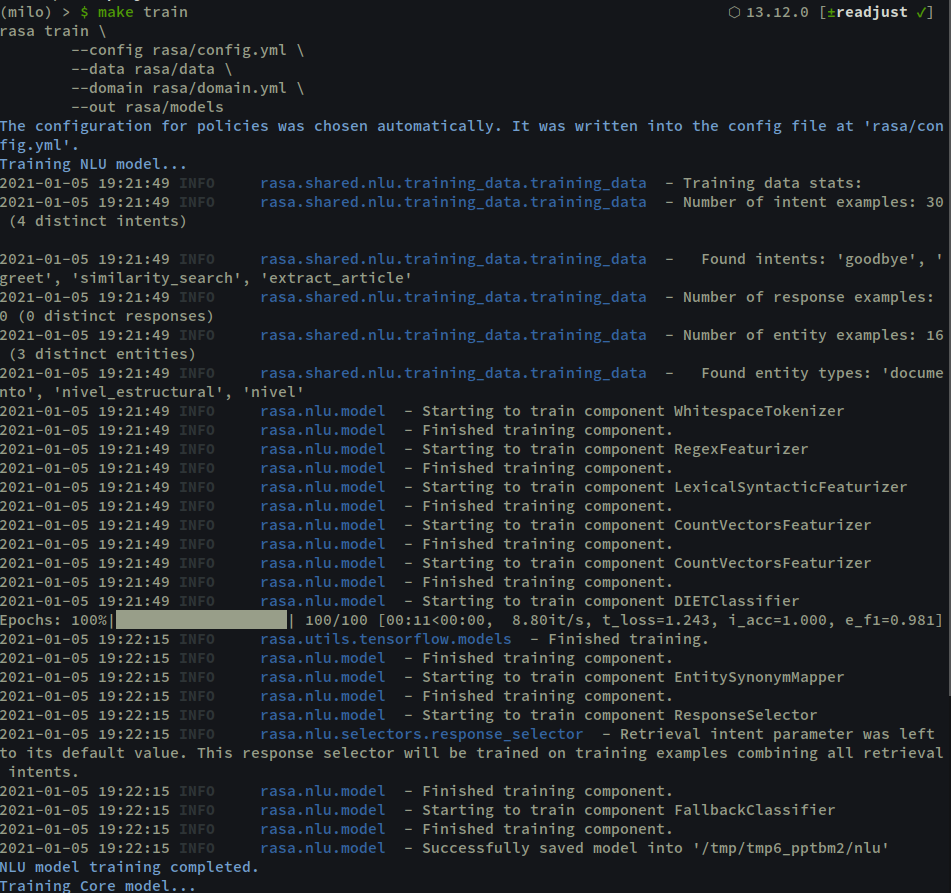
\includegraphics[scale=0.47]{images/6/training}
    \caption{Ejecución del entrenamiento del modelo de clasificación para el intérprete.}
    \label{fig:entrenamiento}
\end{figure}

\subsubsection{Nota adicional sobre los datos de entrenamiento}

Debido a que la naturaleza de este proyecto es la de utilizar conjuntos de datos de conversaciones para el entrenamiento del intérprete, es importante recalcar que constantemente se debe ir refinando con base al funcionamiento del chatbot una vez desplegado; es decir, hacer un contraste sobre los datos utilizados en esta iteración contra futuras evaluaciones con conversaciones reales. Estos datos se deberán ir actualizando en los archivos \href{https://github.com/AranGarcia/milo-bot/blob/master/rasa/data/stories.yml}{stories.yml} y \href{https://github.com/AranGarcia/milo-bot/blob/master/rasa/data/nlu.yml}{nlu.yml} para que Rasa los utilice en el aprendizaje.

\subsection{Implementación de scripts para la preparación de texto}

Para facilitar el proceso de transformación y carga de datos de documentos normativos se desarrollaron dos scripts que automatizan este proceso:

\begin{itemize}
    \item \href{https://github.com/AranGarcia/milo-bot/blob/master/1_preparcion.py}{1\_preparcion.py}:Script de transformación de formato estructurado de TXT a JSON.
    \item \href{https://github.com/AranGarcia/milo-bot/blob/master/2\_carga.py}{2\_carga.py}: Script de carga para poblar la base de conocimientos.
\end{itemize}

\subsubsection{Transformación de formato}
 
 Ayudará a leer los archivos y estructurarlos en un formato adecuado para procesarlo de manera jerárquica. La figura \ref{fig:script-preparacion} muestra la salida de esta ejecución.
 
\begin{figure}
    \centering
    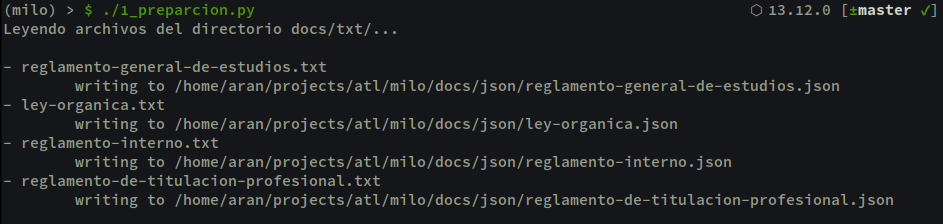
\includegraphics[scale=0.475]{images/6/preparacion}
    \caption{Ejecución del script de preparación.}
    \label{fig:script-preparacion}
\end{figure}


\subsubsection{Carga de datos estructurados}

Este proceso puede ser considerado como el punto de partida en el flujo de proceso para la inicialización del chatbot. A pesar de que el proceso anterior estructura los archivos, es a partir de este proceso se ve ejecuta la solución al problema establecido en este proyecto.

Su propósito es obtener la información estructurada y cargarla en la base datos. También aprovecha para hacer procesamiento del texto introducido y prepararlo a una representación vectorial. A continuación se describe el proceso de manera detallada:

\begin{enumerate}
    \item \textbf{Lectura del vocabulario}
    
    La construcción de las incrustaciones de palabras derivado de un espacio vectorial de palabras ajustado específicamente para el idioma español esta fuera del alcance de este proyecto. Sin embargo, es posible utilizar componentes para procesamiento de lenguaje natural de licencia abierta que sirven de apoyo para proyectos como este.
    
    En primer lugar, necesitamos un modelo de representación vectorial ajustado a nuestro idioma. Se usará los modelos entrenados que proporciona la bibloteca para Python, \textbf{Spacy}. Específicamente hablando, se usará un modelo entrenado con el corpus de texto \href{https://github.com/UniversalDependencies/UD_Spanish-AnCora}{AnCora}. Este corpus tiene metadatos y anotaciones suficientes para el entrenamiento de modelos o procesamiento diverso sobre estructuras sintácticas y gramaticales. Spacy proporciona ya un modelo base entrenado con este corpus y una interfaz de progrmación en donde podemos cargar este modelo y usarlo en nuestro procesamiento.
    
    Segundo, es importante contar con un conjunto de palabras conocidas para considerarlo en nuestro idioma español, junto con la forma lematizada de cada palabra para poder unificar semánticamente las inflexiones de las palabras en un mensaje. El repositorio \textbf{lemmatization-lists} tiene un recopilado de listas en distintos idiomas que incluyen estos lemas. Para este proyecto, se usará el archivo \href{https://github.com/michmech/lemmatization-lists/blob/master/lemmatization-es.txt}{lemmatization-lists} para el idioma español.
    
    \item \textbf{Cálculo de los agrupaciones de palabras}
    
    Una vez obtenido los datos suficientes de modelos lingüisticos en el idioma español, se implementa la reducción del vocabulario que se mencionó en la sección \ref{subsec:reduccion-vocabulario} mediante el algoritmo \textbf{K-Means}.
    
    Primeramente, utilizando el vocabulario de lemas en el paso anterior, pasamos a la representación vectorial cada una de ellas. Posteriormente, se procede a reducir por similitud utilizando 1,000 agrupaciones en donde se promedia un conjunto de vectores y se guardará como una \textit{palabra en nuestro vocabulario}, que en realidad es un grupo de palabras similares.
    
    Cabe mencionar que el vocabulario de lemas contiene \textbf{67620 palabras en su vocabulario} y que los vectores generados a partir del espacio vectorial tienen una dimensión de 300 índices. El procesamiento de estos clusters requiere un tiempo de ejecución de varias horas, aún usando bibliotecas optimizadas para de acceso a memoria por lotes grandes de información y procesamiento sobre ellas, como lo es \textbf{Numpy}. Esto se debe a que la complejidad es de $O(knT)$, en donde $n$ es la cantidad de muestras y $T$ el número de la iteración; sin embargo en el peor de los casos puede llegar a ser de $O(n^{k+2/p})$. Como optimización, el resultado de esta operación se serializa y se guarda en un archivo \href{https://github.com/AranGarcia/milo-bot/commit/f2d1df140d4574b6ceda82b9ba4fbb4d9173d80b#diff-931aebaaaa2cf759c308eb067ebc5b9ea29914278192b98e7d0520a576087dbe}{docs/wv.npy}, el cuál hace que no sea necesario volver a tener que calcularla y distribuirla una única vez.
    
    \item \textbf{Cálculo de la matriz de similitud}
    
    El resultado del paso anterior da las 1,000 agrupaciones semánticas listas para ser utilizadas en nuestro procesamiento. El primer uso que se les da es considerar qué tan similar son cada vector agrupado contra todos los demás; esto también incluye compararlo consigo mismo. Esto es la definición de la matriz que se mencionó en la sección \ref{sec:deteccion-parafrasis}.
    
    Al igual que con el cálculo de agrupaciones, este proceso escribe los datos de manera serializada en un archivo \href{https://github.com/AranGarcia/milo-bot/commit/f4f897e0c58e08faeb48df13aedf71241351215e#diff-fb0888c56c64fe00e47679ff9dade943756c12209861ba9232fa0592f0299a63}{docs/sm.npy}. Sin embargo, este cálculo no requiere tanto tiempo de procesamiento como el paso anterior, pero es una optimización aceptable para este proyecto.
    
    \item \textbf{Lectura del documento a nivel estructural}
    
    Como última instancia, ahora se considera hacer una transformación de los documentos normativos a datos que podremos cargar a la base de conocimientos y poder utilizarla en este proyecto. De manera recursiva, se accede a los niveles estructurales de los documentos legales considerando el \textit{nivel}, la \textit{enumeración}, \textit{el nombre del documento} y por supuesto el mismo \textit{texto} que contiene los reglamentos.
    
    Mas aún, el texto obtenido en cada reglamento pasa por una subrutina para pasarlo a una representación vectorial que se utilizará en búsqueda de conceptos. Este proceso consta de los siguientes pasos:
    
    \begin{enumerate}
        \item Eliminar puntaciones y caracteres que no sean alfanuméricos
        \item Separar las oraciones en palabras.
        \item Obtener la forma lematizada de cada palabra.
        \item Obtener la representación vectorial de la forma lematizada.
        \item Calcular la similitud coseno entre el vector y todas las 1,000 agrupaciones.
        \item Identificar la palabra como perteneciente a esa agrupación.
    \end{enumerate}
    
    La descripción de los pasos anteriores, junto con la construcción de vectores binarios, da como resultado la implementación del algoritmo descrito en la sección \ref{fig:algoritmo-deteccion-parafrasis}.
    
\end{enumerate}

La figura \ref{fig:script-carga} muestra la salida de la ejecución del escript de carga, en dónde se puede notar que previamente se han calculado las agrupaciones o \textit{clusters} de palabras con las que se identificarán semánticamente las palabras de los documentos normativos, así como la matriz de similitud en las que se calcula la similitud coseno entre estas agrupaciones.

\begin{figure}
    \centering
    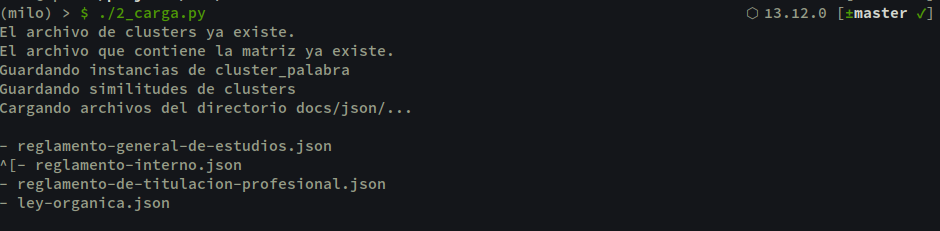
\includegraphics[scale=0.5]{images/6/carga}
    \caption{Ejecución del script de carga a la base de datos.}
    \label{fig:script-carga}
\end{figure}

\section{Tercera iteración}

Como última parte del desarrollo, en esta fase el sistema cuenta con los componentes base con los cuáles el desarrollo puede ejecutarse de manera evolutiva con un diseño para la implementación de funcionalidades.

En este caso, el principal desarrollo consiste en la implementación de las funciones que correspondan a la ejecución de la lógica que atiende las consultas dependiendo del tipo de intención del usuario introducida a través del chat.

Con base a los servicios construidos en las iteraciones pasadas, ahora se necesitan las interfaces de programación para utilizarlos. A grandes rasgos, se tienen dos módulos principales:

\begin{itemize}
    \item \textbf{lib/db.py}: módulo que proporciona la capa de acceso a la fuente de datos para operaciones CRUD.
    \item \textbf{lib/nlputils.py}:
\end{itemize}
 
\subsection{Implementación del módulo de recuperación de texto}



\subsection{Implementación del algoritmo de similitud}
 
% \section{Ajuste adicional: Cuarta iteración}
 
\section{Cuarta iteración}

Descripción del cambio en algoritmo de similitud
 
 \begin{figure}
     \centering
     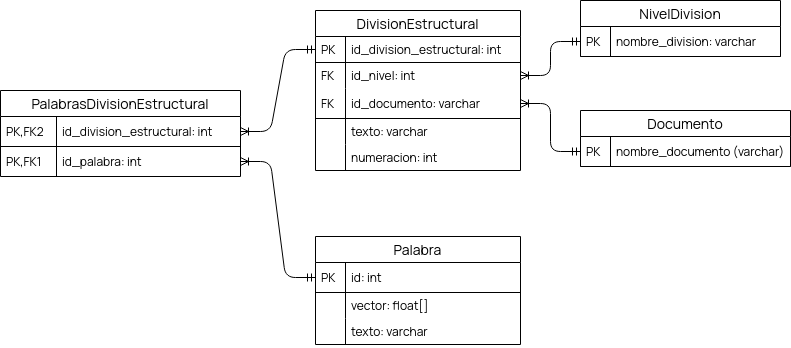
\includegraphics[scale=0.55]{images/6/modelo-relacional-modificado}
     \caption{Modelo de datos modificado.}
     \label{fig:modelo-datos-v2}
 \end{figure}